
\chapter[Методы выбора оптимального местоположения базовых \\станций]{Методы выбора оптимального местоположения \\базовых станций}

Базовая станция~\cite{def-bs} мобильного оператора --- это установка, предназначенная для передачи и приёма радиосигналов между мобильными устройствами и сетью сотовой связи. Она является одним из основных компонентов мобильной сети.

Задача определения оптимального расположения базовых станций заключается в выборе подмножества местоположений для базовых станций, которые обеспечивают подключение в целевой области. 

Целевая область разбивается на элементарные области одинакового размера.

Каждая элементарная область является потенциальной точкой размещения базовой станции и представляет всех потребителей, находящихся на её территории. Каждая элементарная область получает сигнал от всех передатчиков. Элементарная область считается обслуженной, если одна из метрик сигнала в ней выше порогового значения. Рассматриваемая формулировка предполагает, что частота и мощность всех передатчиков одинаковы. 


\section[Содержательная постановка задачи выбора оптимального\\ местоположения базовых станций]{Содержательная постановка задачи выбора\\ оптимального местоположения базовых станций}

Для решения задачи выбора оптимального местоположения базовых станций необходимо подготовить такие параметры базовых станций как радиус покрытия --- максимальный теоретический радиус зоны покрытия БС для связи с устройствами; пропускная способность базовой станции, то есть какой объём данных может передавать станция; стоимость размещения базовой станции.

В беспроводных широкополосных сетях зачастую используются радиоволны сантиметрового диапазона ~\cite{wave-len}. Отличительной чертой распространения таких радиоволн является почти полное отсутствие явления дифракции и прямолинейность распространения. Волны практически не огибают преград при распространении, поэтому существенное влияние на потерю сигнала оказывают рельеф местности, преграды и погодные условия.

Также при размещении базовых станций обязательно должны быть учтены нормы СанПиН~2.1.8/2.2.4.1383-03~\cite{sanpin}. 

Задано множество $T$ элементарных областей, на которые поделена целевая область и с которыми необходимо обмениваться информацией. Также задано множество $B$ мест возможного размещения базовых станций.

С вершинами $T$ необходимо обмениваться информацией. $S = \{s_k\}, k = \overline{1, m}$ --- множество типов размещаемых базовых станций. Каждому типу базовой станции, размещённой на вершине множества $B$ приписаны два параметра $s_k = \{\{r_{ij}\}, c_i\}$, где:
\begin{itemize}
	\item[---] $\{r_{ij}\}$ множество радиусов телекоммуникационного покрытия базовой станции. Параметр $r_{ij}$ характеризует дальность связи между базовой станцией размещенной в вершине $b_i, b_i \in B$ и географическим центром области в вершине, $t_j \in T$;
	\item[---] $c_i$ --- стоимость размещения.
\end{itemize}

Требуется определить набор типов станций минимальной стоимости из множества $S$ и места размещений этих станций на множестве $B$, при условии что каждый из объектов множества $T$ попадает в зону обслуживания, хотя бы одной базовой станции.

\section[Математическая постановка задачи выбора оптимального\\ местоположения базовых станций]{Математическая постановка задачи выбора\\ оптимального местоположения базовых станций}

Рассмотрим математическую постановку задачи. Можно представить задачу в матричном виде. Пусть $W = (w_{(i,k)j})$ --- произвольная матрица с элементами $w_{(i,k)j} \in \{0,1\}$ без нулевых строк и столбцов. Будем говорить, что в $W$ строка $j$ покрывается столбцом $(i,k)$, если $w_{(i,k)j} = 1$.  Подмножество столбцов называется покрытием, если в совокупности они покрывают все строки матрицы $W$. Пусть каждому столбцу поставлено в соответствие положительное число $c_{(i,k)}$ --- стоимость размещения базовой станции типа $k$ на месте $i$. Требуется найти покрытие минимальной стоимости. Вводя переменные $x_{(i,k)}$, равные 1, если столбец $(i,k)$ входит в искомое покрытие, и равные 0 в противном случае, приходим к следующей формулировке задачи: 
\vspace{-5mm}
\begin{equation}
	F = \sum_{i=1}^n\sum_{k=1}^m c_{(i,k)}x_{(i,k)} \rightarrow \min
\end{equation}

при следующих ограничениях.

Каждый объект $t_j$ должен обслуживаться хотя бы одной базовой станцией.

\begin{equation}
	\sum_{i=1}^n\sum_{k=1}^m w_{(i,k)j}x_{(i,k)} \ge 1
\end{equation}

На одном месте $b_i$ может быть размещено не более одной станции.

\begin{equation}
 	\sum_{k=1}^{m} x_{(i,k)} \le 1
\end{equation}

Таким образов задачу выбора оптимального местоположения базовых станций можно представить в виде системы неравенств~\ref{slau}.

\begin{equation}
	\label{slau}
	\begin{cases}
		\begin{array}{ccc}
			w_{(1,1)1}x_{(1, 1)} &+  \cdots  +& w_{(n,m)1}x_{(n,m)} \ge 1\\
			\vdots & \ddots & \vdots\\
			w_{(1,1)l}x_{(1, 1)} &+  \cdots  +& w_{(n,m)l}x_{(n,m)} \ge 1\\
			x_{(1,1)}& +  \cdots  + &x_{(1,m)} \le 1\\
			\vdots & \ddots & \vdots\\
			x_{(n,1)} &+  \cdots  + &x_{(n,m)} \le 1\\
		\end{array}
	\end{cases}
\end{equation}

Для всех областей $t_j$, для которых $w_{ikj} = 1$:
\begin{equation}
	\frac{a_{ikj} x_{ik}}{\mu + \sum a_{ikj} x_{ik}} \ge \delta, 
\end{equation}
где $\beta \in B$, $\tau \in T$, $a_{ikj} > 0$ --- измеренная в $j$ мощность сигнала полученного от станции типа $k$ с места $i$, $\delta \ge 0$ --- нижняя граница SINR, требуемое качество связи, $\mu > 0$ --- шум в системе.

Будем считать что приёмник находится в радиусе телекоммуникационного покрытия базовой станции тогда и только тогда, когда у него будет хорошее качество связи с базовой станцией, то 
есть $\delta \ge 13$дБ. Характеристики качества сигнала~\cite{sinr} приведены в таблице \ref{tbl:sig-quality}.

\captionsetup{justification=raggedright, singlelinecheck=false}
\begin{table}[H]
	\centering
	\begin{threeparttable}
		\caption{\label{tbl:sig-quality}Характеристики качества сигнала с использованием SINR}
		\begin{tabular}{|c|c|}
			\hline
			Качество сигнала & SINR (дБ)\\\hline
			Отличное& $\delta \ge 20$\\\hline
			Хорошее& $13 \ge \delta < 20$ \\\hline
			Среднее& $0 \ge \delta < 13$ \\\hline
			Плохое& $\delta < 0$\\\hline
		\end{tabular}	
	\end{threeparttable}
\end{table}



Для нахождения мощности сигнала между отдельными приёмниками и 
излучателями  используется формула~\cite{atb}:

\begin{equation}
	a_{ikj} = W_{ik} - PL(f, d),
\end{equation}
где $W_{ik}$ --- мощность излучателя базовой станции, $PL(f, d)$ --- потери 
сигнала с расстоянием $d$ на частоте $f$. 

Для расчёта потерь сигнала могут использоваться различные модели.

\subsection{Модель распространения радиоволн SUI}

Рассматривая влияние рельефа местности на качество сигнала~\cite{pl}, можно выделить три категории:
\begin{enumerate}
	\item А --- горная местность, большая растительность или плотная городская застройка с большим количеством препятствий, вследствие чего большие затухания;
	\item B --- горная местность и редкая растительность или пригородная зона с разновысотными постройками; 
	\item С --- плоский рельеф и редкая растительность или сельская местность с малым количеством препятствий, наименьшие затухания.
\end{enumerate}
Данная модель используется для диапазона частот 1900 МГц -- 11 Ггц~\cite{sui}.
Потери сигнала рассчитываются по следующей формуле:
\begin{equation}
	PL(f, d) = 20\lg\frac{4\pi d_0}{\lambda} + 10\gamma\lg\frac{d}{d_0} + X_f + X_h + s, 
\end{equation}
\vspace{-5mm}
\begin{equation}
	\gamma = a - b \cdot h_{bc} + \frac{c}{h_{bc}},
\end{equation}

\begin{equation}
	X_f = 6\lg\frac{f}{2000},
\end{equation}

\begin{equation}
	X_h = 20\lg\frac{h_{ab}}{2}
\end{equation}

где $d_0$ = 100м; $\lambda$ --- длина волны, м; $\gamma$ --- экспонента потерь сигнала мобильной связи, дБ; $d$ --- расстояние от базовой станции до абонентской, м; $h_{bc}$ и $h_{ab}$ --- высоты антенн базовой и абонентской станции, м; $X_f$ --- коэффициент коррекции частоты; $X_h$ --- коэффициенты коррекции высоты приёмника антенны; $f$ – рабочая частота, МГц; $a$, $b$, $c$ --- коэффициенты, зависящие от категории местности согласно таблице~\ref{tbl:place}.

\begin{table}[H]
	\centering
	\begin{threeparttable}
		\caption{\label{tbl:place}Зависимость коэффициентов от 
			категории местности}
		\begin{tabular}{|c|c|c|c|}
			\hline
			Коэффициенты & Категория А & Категория B &Категория C\\\hline
			$a$&4.6&4&3.6\\\hline
			$b$& 0.0075&0.0065&0.005 \\\hline
			$c$& 12.6&17.1&20\\\hline
		\end{tabular}	
	\end{threeparttable}
\end{table}

\subsection{Модель Окамуры---Хата}

Модель распространения Окамура---Хата~\cite{hata} используется для частотного диапазона 150 -- 1500 МГц, расстояние между базовой станцией и абонентским устройством 1 -- 100 метров, высота антенн БС 30--200 метров, высоты антенн абонентских устройств 1 -- 10 метров, дальности телекоммуникационной связи 1--20 км.

Модель Окамура---Хата учитывает особенности территории и плотность застройки: открытая сельская местность, пригородная местность и городская местность. Для каждого случая выражается свой расчёт потерь.

\textbf{Городская местность.}
\begin{equation}
	L_u = 69.55 + 26.16\lg f_c - 13.82 \lg h_b - a(h_m)	+ (44.9 - 6.55 \lg h_b) \lg R,
\end{equation}
\vspace{-8mm}
\begin{equation}
	L_{fs} = L_u
\end{equation}

где $f_c$ --- несущая частота, $h_b$ --- высота антенн базовой станции, $h_m$ – высота антенны абонентского устройства, $a(h_m)$ --- поправочный коэффициент, $R$ --- расстояние между устройствами.

Поправочный коэффициент $a(h_m)$ выражается для малых и средних городов
\begin{equation}
	a(h_m) = (1.1 \lg f_c - 0.7)h_m - (1.56 \lg f_c - 0.8)
\end{equation}

и для больших городов
\begin{equation}
	a(h_m) =
	\begin{cases}
		8.29(\lg (1.54h_m))^2 - 1.1, & 150\text{МГц} \le f_c \le 200\text{МГц},\\
		3.2(\lg (11.75h_m))^2 - 4.97,& 400\text{МГц} \le f_c \le 1500\text{МГц}.
	\end{cases}
\end{equation}

\textbf{Пригородная местность.}
\begin{equation}
	L_{fs} = L_u - 2(\lg(f_c/28))^2 - 5.4
\end{equation}

\textbf{Сельская (открытая) местность.}

\begin{equation}
	L_{fs} = L_u - 4.78(\lg(f_c))^2 + 18.33 \lg(f_c) - 40.94. 
\end{equation}



\section{Методы решения задачи о покрытии}

Рассматриваемая задача является задачей линейного целочисленного программирования, а именно задачей о покрытии множества~\cite{gen-hard}. Задача о покрытии множествами заключается в нахождении набора подмножеств, покрывающего всё множество и имеющего минимально 
возможный вес. Задача о покрытии множества относится к числу NP-трудных. Одними из самых популярных методов решения являются метод полного перебора, генетический алгоритм, метод ветвей и границ~\cite{method-compare}.


\subsection{Генетический алгоритм}

Предложенные в 1975 году Джоном Холландом генетические алгоритмы основаны на принципах естественного отбора и наследования и относятся к стохастическим методам. Эти алгоритмы успешно применяются в различных областях деятельности (экономика, физика, технические науки и т. п.), их используют для решения многих оптимизационных задач. На~\ref{fig:gageneral} представлена общая схема работы генетического алгоритма.

\captionsetup{justification=centering,singlelinecheck=false}
\begin{figure}[H]
	\centering
	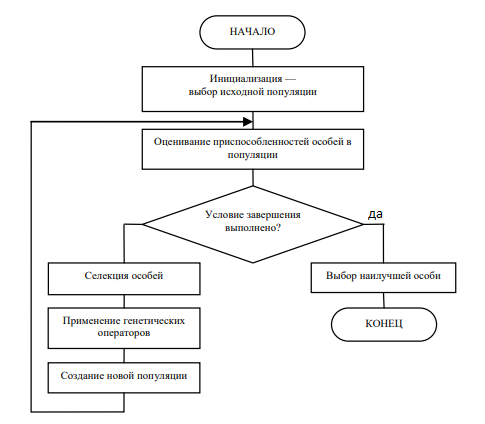
\includegraphics[width=0.7\linewidth]{inc/img/gaGeneral}
	\caption[]{Общая схема генетического алгоритма}
	\label{fig:gageneral}
\end{figure}

Представленная схема является общим алгоритмом для решения многих задач, и при применении её к конкретной задаче необходимо выбрать механизм кодирования параметров в гены особи, оптимизационную функцию, условие останова~\cite{genetic}. Авторы модифицировали модель Голдберга и применили её для решения задачи покрытия множеств. В данном случае оптимизационной функцией будет являться минимизация веса покрытия, а условием останова будет неизменность лучшего решения в течение заданного числа поколений. 

Рассмотрим механизм кодирования особи. Каждый индивид $k$ представлен хромосомой, являющейся $n$-мерным вектором $x^k$, у которого $j$-й элемент $x^k_j$ принимает значение 1, если подмножество $S_j$ входит в покрытие, и принимает значение 0, если иначе.

С таким представлением степень приспособленности $f_k$ индивида $x^k$ может быть рассчитана следующим образом:
\vspace{-5mm}
\begin{equation}
	f_k = \sum_{j=1}^{n} c_{j}x^k_j,
\end{equation}

где $c_j$ — стоимость подмножества $S_j$.

Таким образом, оптимизационная функция выглядит как $f_k \rightarrow \min$.

Для выбора родительских особей используется случайный отбор. В алгоритме используется тип мутации, основанный на изменении случайного гена на противоположное значение. Оператор скрещивания точечный. Выбираются пары хромосом из родительской популяции. Далее для каждой пары отобранных таким образом родителей разыгрывается позиция гена (локус) в хромосоме, определяющая так называемую точку скрещивания --- $l_k$. В результате скрещивания пары родительских хромосом получается следующая пара потомков: $P_1$ — потомок, хромосома которого на позициях от 1 до $l_k$ состоит из генов первого родителя, а на позициях от $l_k + 1$ до $L$ --- из генов второго родителя; $P_2$ — потомок, хромосома которого на позициях от 1 до $l_k$ состоит из генов второго родителя, а на позициях от $l_k + 1$ до $L$ --- из генов первого родителя. 

Начальное поколение состоит из особей, сформированных случайно с помощью алгоритма, подобному жадному алгоритму.

Очень важная деталь работы генетического алгоритма в том, что при скрещивании и мутации могут появится особи, соответствующие покрытия которых не существуют, то есть получаются недопустимые решения. Алгоритм проверяет, существует ли покрытие, и если нет, то пытается, в случае скрещивания, выбрать другую вторую родительскую особь, а в случае мутации — выбрать другой ген для его инвертирования. Если и это не «исправит» особь, родитель выбирается заново случайным образом. Потомок заменяет случайно выбранную особь, если его приспособленность выше.

Рассмотрим на примере, как работает генетический алгоритм и как он избавляется от недопустимых решений. Задача представлена в виде матрицы размером 10x10, заполненной <<0>> и <<1>>. Столбцы матрицы — это подмножества  множества $U$, а строки --- элемента множества $U$. Таким образом, множество $U = \{x_0,\cdots,x_9\}$, и оно состоит из 10 подмножеств $S=\{S_0,\cdots,S_9\}$. <<1>> в матрице обозначает, что соответствующее столбцу подмножество покрывает соответствующий строке элемент.

\captionsetup{justification=raggedright, singlelinecheck=false}
\begin{table}[H]
	\centering
	\begin{threeparttable}
		\caption{\label{tbl:gaex}Матрица подмножеств исходного множества}
		\begin{tabular}{|c|c|c|c|c|c|c|c|c|c|c|}
			\hline
			&S0& S1& S2& S3& S4& S5& S6& S7& S8& S9 \\\hline
			x0& 0& 1& 0& 0& 1& 0& 1& 1& 1& 1\\\hline
			x1& 1& 0& 1& 0& 1& 1& 0& 0& 1& 0\\\hline
			x2& 0& 1& 0& 1& 0& 0& 1& 1& 0& 1\\\hline
			x3& 1& 0& 1& 0& 1& 1& 0& 1& 0& 0\\\hline
			x4& 1& 1& 0& 1& 0& 1& 1& 1& 0& 0\\\hline
			x5& 0& 0& 1& 1& 0& 0& 0& 0& 0& 1\\\hline
			x6& 1& 0& 0& 0& 1& 0& 1& 0& 1& 0\\\hline
			x7& 0& 0& 1& 0& 1& 0& 0& 0& 0& 1\\\hline
			x8& 0& 0& 1& 1& 1& 1& 0& 1& 0& 1\\\hline
			x9& 0& 1& 1& 0& 1& 0& 1& 1& 1& 1\\\hline
		\end{tabular}
	\end{threeparttable}
\end{table}



Используем для поиска покрытия генетический алгоритм с 10 особями.
Каждая особь соответствует определённому покрытию, поэтому длина особи равна 10 и каждый ген
$Ch=\{Ch_0,\cdots,Ch_9\}$ соответствует определённому подмножеству. Если ген особи равен "1", то подмножество входит в покрытие, если <<0>>, то не входит.

На начальном шаге алгоритма особи формируются случайным образом. Представим особи и их гены в виде 
массива, где строка --- особь, столбец --- ген особи.

\captionsetup{justification=raggedright, singlelinecheck=false}
\begin{table}[H]
	\centering
	\begin{threeparttable}
		\caption{\label{tbl:genex}Формирования начальной популяции}
		\begin{tabular}{|c|c|c|c|c|c|c|c|c|c|c|}
			\hline
&$Ch_0$& $Ch_1$& $Ch_2$& $Ch_3$& $Ch_4$& $Ch_5$& $Ch_6$& $Ch_7$& $Ch_8$& $Ch_9$\\\hline
особь 0& 1& 1& 1& 0& 0& 0& 0& 0& 0& 0\\\hline
особь 1& 1& 0& 0& 0& 1& 0& 0& 0& 0& 1\\\hline
особь 2& 1& 0& 0& 1& 0& 1& 0& 0& 0& 1\\\hline
особь 3& 1& 1& 1& 0& 0& 0& 0& 1& 0& 0\\\hline
особь 4& 0& 0& 0& 1& 1& 0& 1& 0& 0& 0\\\hline
особь 5& 1& 0& 0& 1& 1& 0& 0& 0& 0& 0\\\hline
особь 6& 0& 0& 0& 0& 0& 0& 0& 0& 0& 0\\\hline
особь 7& 1& 0& 1& 0& 0& 1& 0& 1& 0& 1\\\hline
особь 8& 0& 0& 0& 1& 1& 0& 1& 1& 0& 0\\\hline
особь 9& 1& 1& 1& 0& 0& 1& 0& 0& 1& 0\\\hline
		\end{tabular}
\end{threeparttable}
\end{table}

На следующем шаге случайно выбрана родительская особь 1. С некоторой вероятностью к ней применяется оператор одноточечного скрещивания, поэтому случайно выбирается вторая родительская особь 2. Точка скрещивания = ген №3. После скрещивания получаем потомка:

\begin{table}[H]
	\centering
	\begin{threeparttable}
		\begin{tabular}{|c|c|c|c|c|c|c|c|c|c|}
			\hline
			1& 0& 0& 0& 0& 1& 0& 0& 0& 1 \\\hline
		\end{tabular}
	\end{threeparttable}
\end{table}

Покрытие, соответствующее этому потомку, существует. С некоторой вероятностью к потомку применяется оператор одноточечной мутации. Случайным образом выбран ген №9, он меняет своё значение на противоположное.
\begin{table}[H]
	\centering
	\begin{threeparttable}
		\begin{tabular}{|c|c|c|c|c|c|c|c|c|c|}
			\hline
			1& 0& 0& 0& 0& 1& 0& 0& 0& 0 \\\hline
		\end{tabular}
	\end{threeparttable}
\end{table}
Но такого покрытия не существует, алгоритм пытается выбрать другой ген, выбран ген №2.

Особь-потомок:
\begin{table}[H]
	\centering
	\begin{threeparttable}
		\begin{tabular}{|c|c|c|c|c|c|c|c|c|c|}
			\hline
			1& 0& 1& 0& 0& 1& 0& 0& 0& 1 \\\hline
		\end{tabular}
	\end{threeparttable}
\end{table}

Такое покрытие существует. Далее в поколении случайно выбирается особь №9, которую, возможно, заменит потомок. Приспособленность потомка равная 4 выше приспособленности особи №9 равной 5, поэтому он её заменяет.

Все описанные шаги выбора родительских особей и применения к ним операторов скрещивания и мутации повторяются, пока не будет найдено решение. Алгоритм заканчивает свою работу, если решение не может быть улучшено за заданное число поколений.

\subsection{Алгоритм полного перебора}

Полный перебор --- точный метод решения оптимизационных задач, относящийся к классу методов поиска решения исчерпыванием всевозможных вариантов. Сложность полного перебора зависит от количества всех возможных решений задачи. 

Полным перебором можно решить любую задачу из класса NP-полных задач. В зависимости от количества всех возможных решений задачи и времени вычисления целевой функции от каждого решения полный перебор может потребовать экспоненциального времени работы.

Идея алгоритма полного перебора для решения задачи покрытия заключается в следующем:
\begin{enumerate}
	\item Поиск всех возможных сочетаний подмножеств исходного множества и сравнение их целевых функций
	\item Определение покрытий среди найденных сочетаний.
	\item Нахождение покрытия минимального веса.
\end{enumerate}

Из теории множеств известно, что число всех подмножеств множества из n элементов равно $2^n$

\subsection{Метод ветвей и границ}
 
Данный метод является модификацией алгоритма полного перебора, что гарантирует точность результата его работы. Суть метода заключается в построении дерева полного перебора и отсечении бесперспективных ветвей решения по мере его обхода, что существенно уменьшает время его работы~\cite{mvig_app}. 
Дерево перебора в этом случае строится так, что на каждом уровне $k$ для каждого из узлов $k-1$ уровня добавляются в качестве дочерних узлов все возможные варианты $a_{kj}x_j$. Для поставленной задачи на каждом уровне добавляется количество узлов, равное количеству $a_{kj}\ne0$. Алгоритм полного перебора предполагает полный обход такого дерева. Алгоритм после обработки каждого узла $k$-ого уровня приступает к обработке дочерних узлов прежде, чем переходит к следующему узлу $k$-ого уровня. Метод ветвей и границ сокращает время поиска оптимального решения за счет того, что при вхождении в каждый узел выполняется верхняя и/или нижняя оценка возможного решения, к которому приведет обход поддерева, корнем которого является текущий узел. В соответствии с полученной оценкой делается вывод --- если лучшее из возможных решений хуже текущего, то данное поддерево (ветвь) отсекается и обход продолжается со следующего узла того же уровня, на котором было произведено отсечение.

Таким образом, ключевым аспектом работы алгоритма по методу ветвей и границ является эффективная оценка поддерева, обязательным требованием к которой также является недопустимость потери точности. Поскольку алгоритм оценки поддерева опирается на текущее решение, инициализация начального решения оставляется на усмотрение разработчика. Возможны четыре варианта инициализации:
\begin{enumerate}
\item Заполнение решения максимальными значениями.
\item Выбор случайного покрытия.
\item Последовательная инициализация лучшими значениями.
\item Нахождение решения приближенным алгоритмом.
\end{enumerate}

Пусть $N$ --- текущее решение задачи, то есть минимальное найденное количество подмножеств Si, покрывающих исходное множество $U$. В таком случае, минимальное улучшение равняется $N-1$. Текущим состоянием M назовём число подмножеств $S_i$, покрывающих сформированный на данном этапе набор. При $M=N-1$ выполняется проверка: если среди непокрытых переменных есть хотя бы одна, которая не покрывается подмножествами $S_i$, формирующими состояние $M$, то минимальное улучшение невозможно, следовательно, данная ветвь считается бесперспективной и отбрасывается. В противном случае текущее состояние $M$ становится текущим решением задачи.

\captionsetup{justification=centering,singlelinecheck=false}
\begin{figure}[H]
	\centering
	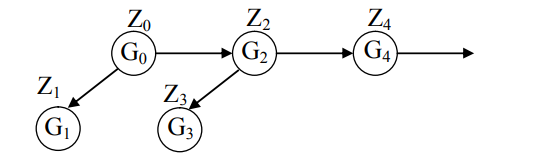
\includegraphics[width=0.7\linewidth]{inc/img/mvig}
	\caption[]{Метод ветвей и границ}
	\label{fig:mvig}
\end{figure}

\chapter[Классификация методов выбора оптимального\\ местоположения базовых станций]{Классификация методов выбора оптимального \\местоположения базовых станций}

В качестве критериев классификации были выбраны такие критерии, как точность и вычислительная сложность.

В таблице~\ref{tbl:class} приведена классификация алгоритмов полного перебора, метода ветвей и границ~\cite{mvig_class} и генетического алгоритма~\cite{gen-hard}.
\captionsetup{justification=raggedright,singlelinecheck=false}
\begin{table}[H]
	\centering
	\begin{threeparttable}
		\caption{\label{tbl:class}Формирования начальной популяции}
		\begin{tabular}{|c|c|c|c|}
			\hline
			Критерий &Алгоритм пол-& Метод ветвей& Генетический \\
			&ного перебора& и границ&алгоритм\\\hline
			Вычислительная &&&\\
			сложность&$O(n!)$&$O(n^5\log_2(n))$&$O(n*m)$\\\hline
			Точность&Точный&Точный&Приближенный\\\hline
		\end{tabular}
	\end{threeparttable}
\end{table}

Из таблицы можно сделать вывод, что генетический алгоритм применим, когда покрыть связью большую площадь. Метод ветвей и границ из-за большой вычислительной сложности применим в тех случаях, где необходимо обеспечить связью небольшой район. 
